\documentclass[tikz]{standalone}

%%% Packages
\usepackage{tikz}
\usetikzlibrary{arrows, positioning, shapes, snakes}


%%% Variables
\newcommand{\minwidth}{3cm}
\newcommand{\minheight}{1cm}


%%% tikzstyle
\tikzstyle{startstop} = [% start stop node
  ellipse,
  minimum width=\minwidth,
  minimum height=\minheight,
  text centered,
  draw=black,
  fill=red!20
  ]
\tikzstyle{io} = [% input output node
  trapezium,
  trapezium left angle=70,
  trapezium right angle=110,
  minimum width=\minwidth,
  minimum height=\minheight,
  text centered,
  draw=black,
  fill=blue!20
  ]
\tikzstyle{process} = [% process node
  rectangle,
  minimum width=\minwidth,
  minimum height=\minheight,
  text centered,
  draw=black,
  fill=orange!20
  ]
\tikzstyle{decision} = [% decision node
  diamond,
  minimum width=\minwidth,
  minimum height=\minheight,
  text centered,
  draw=black,
  fill=green!20
  ]
\tikzstyle{arrow} = [% arrow format
  thick,
  ->,
  >=stealth
  ]


%%%%%%%%%%%%%%%%%%%%%%%%%%%%%%%%%%%%%%%%%%%%%%%%%%%%%%%%%%%%%%%%%%%%%%%%%%%%%%%
\begin{document}

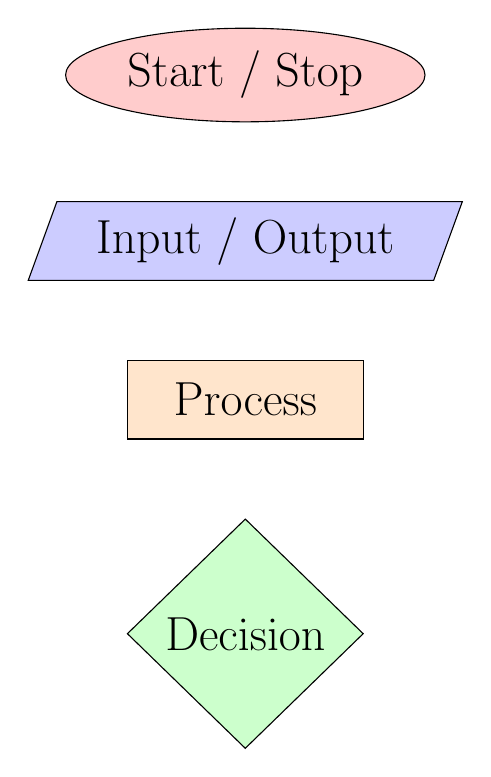
\begin{tikzpicture}[node distance=1cm]

%%% Nodes
\node[startstop] (startstop) {\LARGE Start / Stop};
\node[io] (io) [below=of startstop] {\LARGE Input / Output};
\node[process] (process) [below=of io] {\LARGE Process};
\node[decision] (decision) [below=of process] {\LARGE Decision};

\end{tikzpicture}

%%%%%%%%%%%%%%%%%%%%%%%%%%%%%%%%%%%%%%%%%%%%%%%%%%%%%%%%%%%%%%%%%%%%%%%%%%%%%%%
\end{document}
